\section{Framework Overview}

PrismMathQA is designed as an agentic tutoring framework rather than a single prompt template. The central model is an OpenAI-compatible reasoning LLM that produces the final student-facing explanation. Around it, the framework adds three forms of support: retrieval-augmented generation for mathematical grounding, learner memory for personalization across turns, and symbolic tool calling for exact computation. These components solve different problems and are intentionally complementary. RAG gives the model relevant examples, memory gives it student context, and tool use gives it reliable computation.

\begin{figure}[t]
\centering
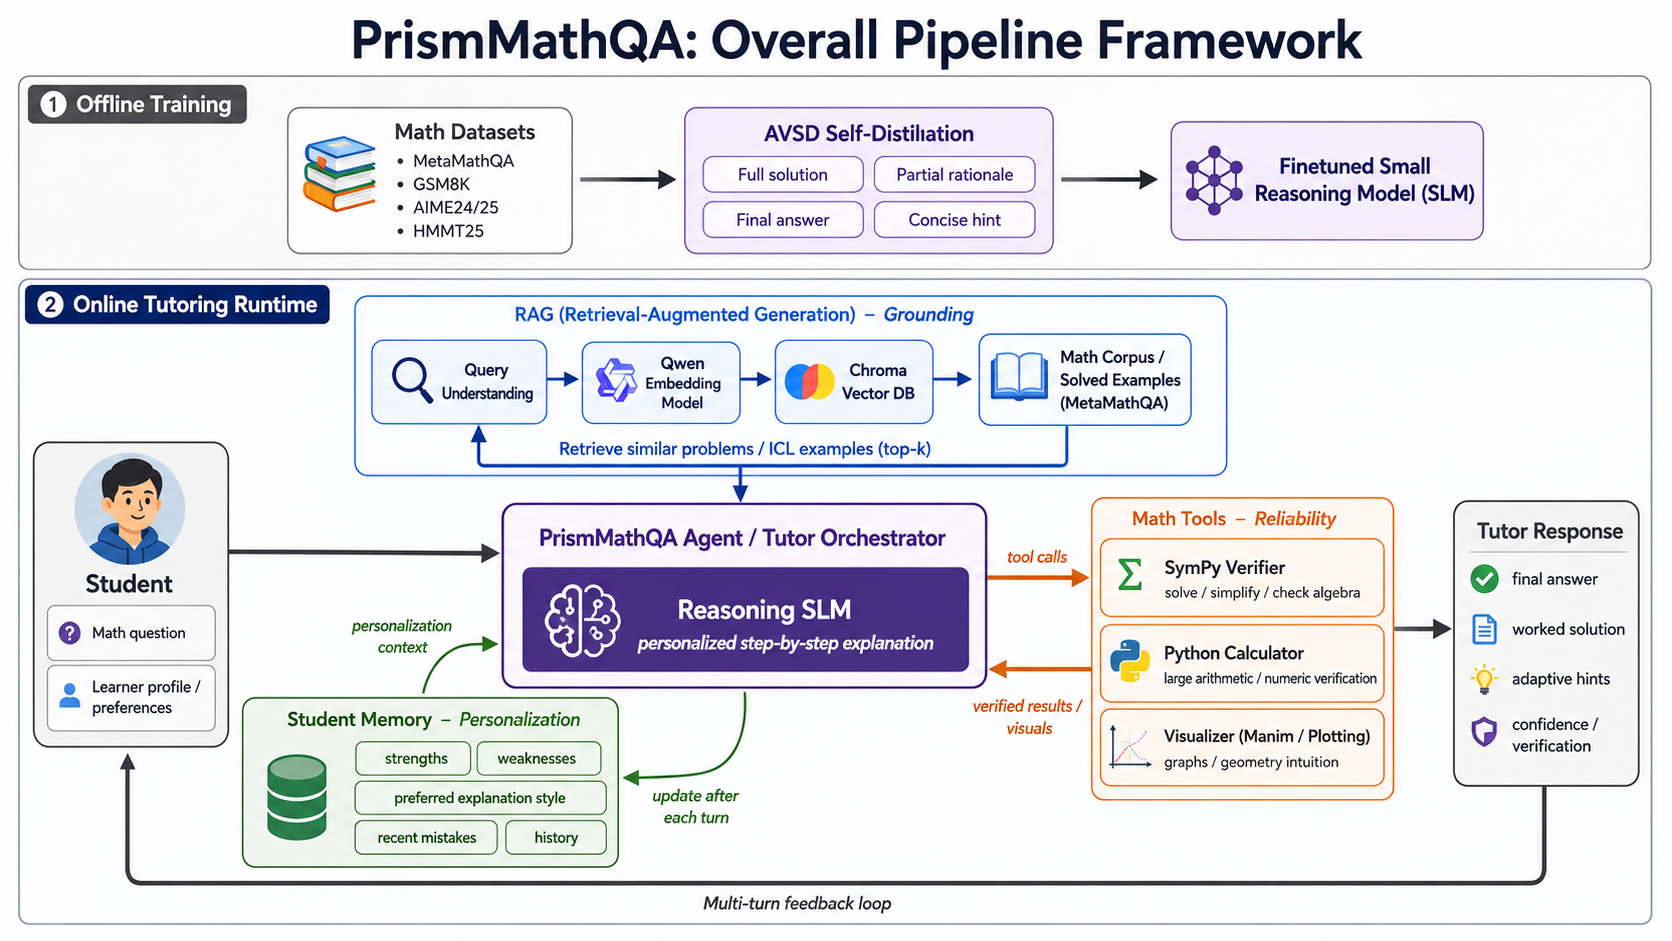
\includegraphics[width=0.82\linewidth]{imgs/prism_mathqa_pipeline.png}
\caption{Overall PrismMathQA pipeline: AVSD trains the reasoning model offline, while RAG, memory, and math tools support the online tutor.}
\label{fig:prismmathqa-pipeline}
\end{figure}

Figure~\ref{fig:prismmathqa-pipeline} shows how the framework separates model training from tutoring-time orchestration. Offline, mathematical datasets are converted into four AVSD views: full solution, partial rationale, final answer, and concise hint. This produces the finetuned reasoning model used by the tutor. Online, the student question is grounded through RAG, adapted through learner memory, and checked through math tools before a final response is returned. The current implementation focuses on retrieval, memory, and symbolic verification; the calculator and visualizer blocks indicate natural extensions for future numerical and geometry-heavy tutoring tasks.

\subsection{Agentic Components}

In ordinary question answering, the model receives only the current prompt and must rely on its parametric knowledge. That setup is fragile for tutoring. A student may ask a problem whose solution depends on a contest-math pattern; the model may know the pattern but fail to recall the right derivation. The same student may then ask follow-up questions that require continuity. Finally, even if the reasoning plan is correct, a small arithmetic error can damage trust. PrismMathQA addresses these issues by separating the tutoring task into agentic components.

The first component is the \emph{reasoning model}. It is responsible for language, pedagogy, and mathematical explanation. It decides how much detail to show, how to adapt to the learner, and how to turn retrieved examples or tool outputs into a coherent response. The second component is the \emph{retrieval module}, which searches a math corpus for semantically similar solved examples. The third component is \emph{memory}, which keeps track of learner preferences and recent interaction history. The fourth component is a \emph{symbolic verification tool}, which checks exact algebra or arithmetic when the model should not rely on free-form generation.

These components are not independent add-ons. They form a division of labor. The reasoning model is strongest at natural language explanation and at connecting mathematical steps into a coherent narrative. The retriever is strongest at finding analogous problems and solution patterns. Memory is strongest at carrying learner-specific context across turns. The symbolic tool is strongest at deterministic computation. PrismMathQA uses the LLM as the coordinator, but it does not require the LLM to solve every subproblem alone. This is the main reason the framework is agentic: the answer is produced through controlled interaction between specialized sources of support.

\subsubsection{Retrieval-Augmented Generation}

RAG is important because mathematical reasoning is highly pattern-sensitive \citep{lewis2020rag}. A problem about a parameterized curve, a geometry perimeter, or a polynomial factorization often resembles earlier worked examples. If the model receives relevant examples in context, it can align its explanation style and decomposition strategy with the target domain. This does not mean that retrieved examples replace reasoning. In PrismMathQA, retrieved examples act as demonstrations: they help the LLM choose a useful solution pattern, but the final answer must still solve the student's exact question.

The retrieval corpus is based on MetaMathQA, a large collection of mathematical question-answer pairs and worked solutions. PrismMathQA embeds questions with Qwen3-Embedding-4B and stores the resulting vectors in Chroma. At inference time, the student's question is embedded with the same embedder, nearest examples are retrieved, and the reasoning model receives them as in-context demonstrations. This design gives the tutor domain-specific mathematical context without requiring the base LLM to memorize every example.

Using Qwen3-Embedding-4B as the embedder is useful because the retriever should understand mathematical semantics rather than only surface-level word overlap. Two problems can share a solution strategy even when their wording is different. For example, a quadratic vertex problem and a completing-the-square example may not share many tokens, but they are close in mathematical structure. Dense embeddings help retrieve by conceptual similarity, while Chroma provides a practical vector-search backend for storing and querying those representations.

In PrismMathQA, retrieval is especially valuable for medium and hard problems. Easy arithmetic questions may not need retrieved context, but contest-style problems often require choosing the right representation. RAG can expose whether a problem should be approached by parameter elimination, factoring, coordinate distance formulas, modular arithmetic, or completing the square. This helps the model choose a starting point before it begins to write the explanation.

\begin{table}[t]
\centering
\caption{Representative MetaMathQA-style examples and why they are useful as a PrismMathQA retrieval corpus.}
\label{tab:metamathqa-corpus}
\small
\begin{tabular}{p{0.16\linewidth}p{0.30\linewidth}p{0.18\linewidth}p{0.18\linewidth}}
\toprule
Question type & Concrete sample question & Mathematical skill & Why it supports RAG tutoring \\
\midrule
Algebraic manipulation & Solve for $x$: $987654321x-123456789=555555555$. Give the answer as a reduced fraction. & Linear equations, exact arithmetic, fraction reduction. & Retrieves examples that show clean symbolic transformations and exact intermediate steps. \\
\midrule
Geometry and coordinate reasoning & A hexagon has consecutive vertices \((0,1)\), \((1,2)\), \((2,2)\), \((2,1)\), \((3,1)\), \((2,0)\), and \((0,1)\). If the perimeter is $a+b\sqrt{2}+c\sqrt{5}$, find $a+b+c$. & Distance formula, radical simplification, geometric modeling. & Retrieves demonstrations that translate diagrams or coordinates into algebraic quantities. \\
\midrule
Functions and graph interpretation & Given $f(x)=x^2-4x+1$, find the vertex, axis of symmetry, and minimum value. & Completing the square, quadratic interpretation. & Supplies high-school level explanations that connect algebraic manipulation to graph meaning. \\
\midrule
Advanced contest reasoning & A curve is $(x,y)=(2\cos t-\sin t,64\sin t)$ and can be written as $ax^2+bxy+cy^2=1$. Find $(a,b,c)$. & Parameter elimination, trigonometric substitution, implicit forms. & Gives harder multi-step patterns where in-context solution structure is especially valuable. \\
\bottomrule
\end{tabular}
\end{table}

Table~\ref{tab:metamathqa-corpus} illustrates why MetaMathQA is appropriate for PrismMathQA. The corpus is not just a list of short arithmetic questions. It contains diverse mathematical structures: symbolic equations, coordinate geometry, function analysis, and competition-style derivations. This diversity matters because the retriever can supply examples at different levels of abstraction. For an easy quadratic problem, a simple worked example may be enough. For a harder parametric curve problem, the system needs examples that demonstrate how to introduce variables, eliminate parameters, and present a final symbolic form.

MetaMathQA is also suitable because its examples include both questions and solution text. A retrieval corpus for tutoring should not only retrieve the answer; it should retrieve a style of reasoning. The model can observe how a solution is broken into steps, how notation is introduced, and how the final result is justified. This makes the corpus useful as an in-context teaching source, not merely as an answer lookup table.

The corpus is also compatible with AVSD. The same mathematical artifacts that make MetaMathQA useful for RAG also make it useful for multi-context finetuning. A worked solution can be transformed into a full-solution view, a truncated partial-solution view, a final-answer view, or a concise hint. This means the runtime retrieval corpus and the training-time privileged views are aligned: both are built from solved mathematical examples, but they are used differently. At inference time, examples are retrieved as demonstrations. During finetuning, the same type of data can provide teacher views for token-level supervision.

\subsubsection{Memory}

Memory is important because tutoring is a longitudinal interaction. A model that forgets the learner after every turn cannot adapt its explanation style or build on prior clarification. PrismMathQA uses memory to represent two kinds of context. The first is a learner profile: grade level, preferred explanation style, strengths, and weak areas. The second is recent conversation history: previous questions, model answers, and tool or retrieval traces.

At a high level, memory solves three problems. First, it supports personalization. A student who asks for step-by-step explanations should receive a different response from a student who wants concise verification. Second, it supports continuity. If the student asks ``why did you divide by this term?'' the tutor needs the previous answer to interpret the follow-up. Third, it supports accountability. Stored interaction summaries make it possible to audit what the tutor saw and how it responded.

Memory is particularly important for mathematics because student errors are often systematic. A learner may repeatedly confuse distribution with factoring, forget sign changes when moving terms across an equation, or apply the power rule incorrectly. Even lightweight memory can help the tutor notice that the student is asking related questions and should receive a targeted reminder. Without memory, the model treats each query as isolated and may miss the opportunity to reinforce the same misconception across examples.

PrismMathQA deliberately keeps memory lightweight. It does not require a complex student model to be useful. Even recent-turn memory can improve tutoring quality because many mistakes and follow-up questions are local. A future version can extend this into mastery tracking, misconception detection, and curriculum recommendation. The current framework treats memory as a necessary context layer that helps the reasoning model behave like a tutor rather than a stateless calculator.

There is also a pedagogical reason to keep memory interpretable. If the system adapts its explanation, the adaptation should be understandable: the tutor is using the learner's stated grade level, preferred style, or recent mistakes. An opaque memory representation may improve performance but can make the tutor harder to audit. PrismMathQA therefore treats memory as a readable context layer first, and a target for richer learner modeling second.

\subsubsection{Tool Calling}

Tool calling is important because mathematical fluency and exact computation are not the same ability. A reasoning LLM can explain a method correctly and still make an arithmetic error. In a tutoring system, this is costly: students may learn the wrong result or lose trust in the explanation. PrismMathQA therefore gives the model access to a symbolic verification tool based on SymPy \citep{meurer2017sympy}.

The tool is used when exact computation materially improves correctness: solving equations, simplifying expressions, checking nontrivial fractions, differentiating or integrating symbolic expressions, or verifying large arithmetic. The reasoning model decides whether a problem should be answered directly or whether a tool call is warranted. If the tool is used, the result is returned to the model, and the model turns that result into a student-facing explanation.

The decision to call a tool is itself part of the tutoring behavior. A good tutor should not outsource every step, because students need to see reasoning. At the same time, a good tutor should not pretend that mental arithmetic is reliable for very large numbers. PrismMathQA therefore uses tool calling selectively. Routine conceptual explanations can remain direct, while exact symbolic or numerical checks can be delegated to the verifier. This preserves the educational role of the LLM while improving factual reliability.

This separation is useful pedagogically. The tool should not replace the explanation; it should stabilize it. For example, when solving a large linear equation, SymPy can verify the exact rational solution, while the LLM explains why adding a term to both sides and reducing a fraction are valid steps. The student sees a coherent solution, but the system has reduced the risk of silent computational error.

Tool calling also creates an audit trail. If an answer depends on a computed derivative or a reduced fraction, the framework can record that the symbolic verifier was used. This matters when evaluating a tutoring system: an evaluator can distinguish between an answer that came from model-only reasoning and an answer that was supported by exact computation. The distinction is useful for debugging, for measuring tool-call appropriateness, and for deciding which failures require better prompting, better tool schemas, or better model training.
